% =====================================================================
\section{Tập dữ liệu và tiền xử lý}
\label{sec:data}
% =====================================================================

\subsection{Dữ liệu và ánh xạ nhãn}
\label{sec:data-mapping}

CIFAR-10 gồm 60.000 ảnh RGB kích thước $32 \times 32$: 50.000 ảnh train chính thức và 10.000
ảnh test chính thức; mỗi lớp gốc có 5.000 ảnh train và 1.000 ảnh test~\cite{krizhevsky2009cifar}.
Hai siêu lớp dưới đây là \emph{phép gộp của đề tài}, không phải bộ nhãn siêu lớp chính thức
của CIFAR-10. Việc ghi rõ điều này là cần thiết để tránh so sánh sai với các bảng xếp hạng
chuẩn.

\begin{table}[htbp]
  \centering
  \small
  \begin{tabular}{@{}c l l c@{}}
    \toprule
    Nhãn mới & Siêu lớp & Các lớp gốc & Số lớp gốc \\
    \midrule
    0 & Animal  & bird, cat, deer, dog, frog, horse & 6 \\
    1 & Vehicle & airplane, automobile, ship, truck & 4 \\
    \bottomrule
  \end{tabular}
  \caption{Ánh xạ từ 10 lớp gốc của CIFAR-10 sang hai siêu lớp của đề tài. Theo thứ tự nhãn gốc,
  Animal $= \{2,3,4,5,6,7\}$ và Vehicle $= \{0,1,8,9\}$.}
  \label{tab:label-map}
\end{table}

Sau ánh xạ, tỷ lệ Animal/Vehicle là $60\,\%/40\,\%$ và không còn cân bằng. Hệ quả trực tiếp:
một bộ phân loại luôn đoán \enquote{Animal} đã đạt Accuracy $60\,\%$ trên phép chia này, nên
Accuracy đơn lẻ không phản ánh chất lượng của lớp thiểu số. Do đó \textbf{Macro-F1 là chỉ số
chính} và Accuracy chỉ là chỉ số bổ sung~\cite{guo2017calibration}.

\figref{fig:dataset-samples} minh họa trực tiếp phép gộp này: mỗi hàng là một lớp gốc, màu
khung thể hiện siêu lớp mà lớp đó thuộc về. Hình cũng cho thấy vì sao bài toán không tầm
thường: cùng một siêu lớp chứa các đối tượng rất khác nhau (chim, mèo, hươu, chó, ếch, ngựa),
trong khi hai siêu lớp lại có thể trông gần giống nhau ở kích thước ảnh $32 \times 32$ — ví dụ
\emph{airplane} nằm trên nền trời xanh có thể bị nhầm với \emph{bird}.

\begin{figure}[htbp]
  \centering
  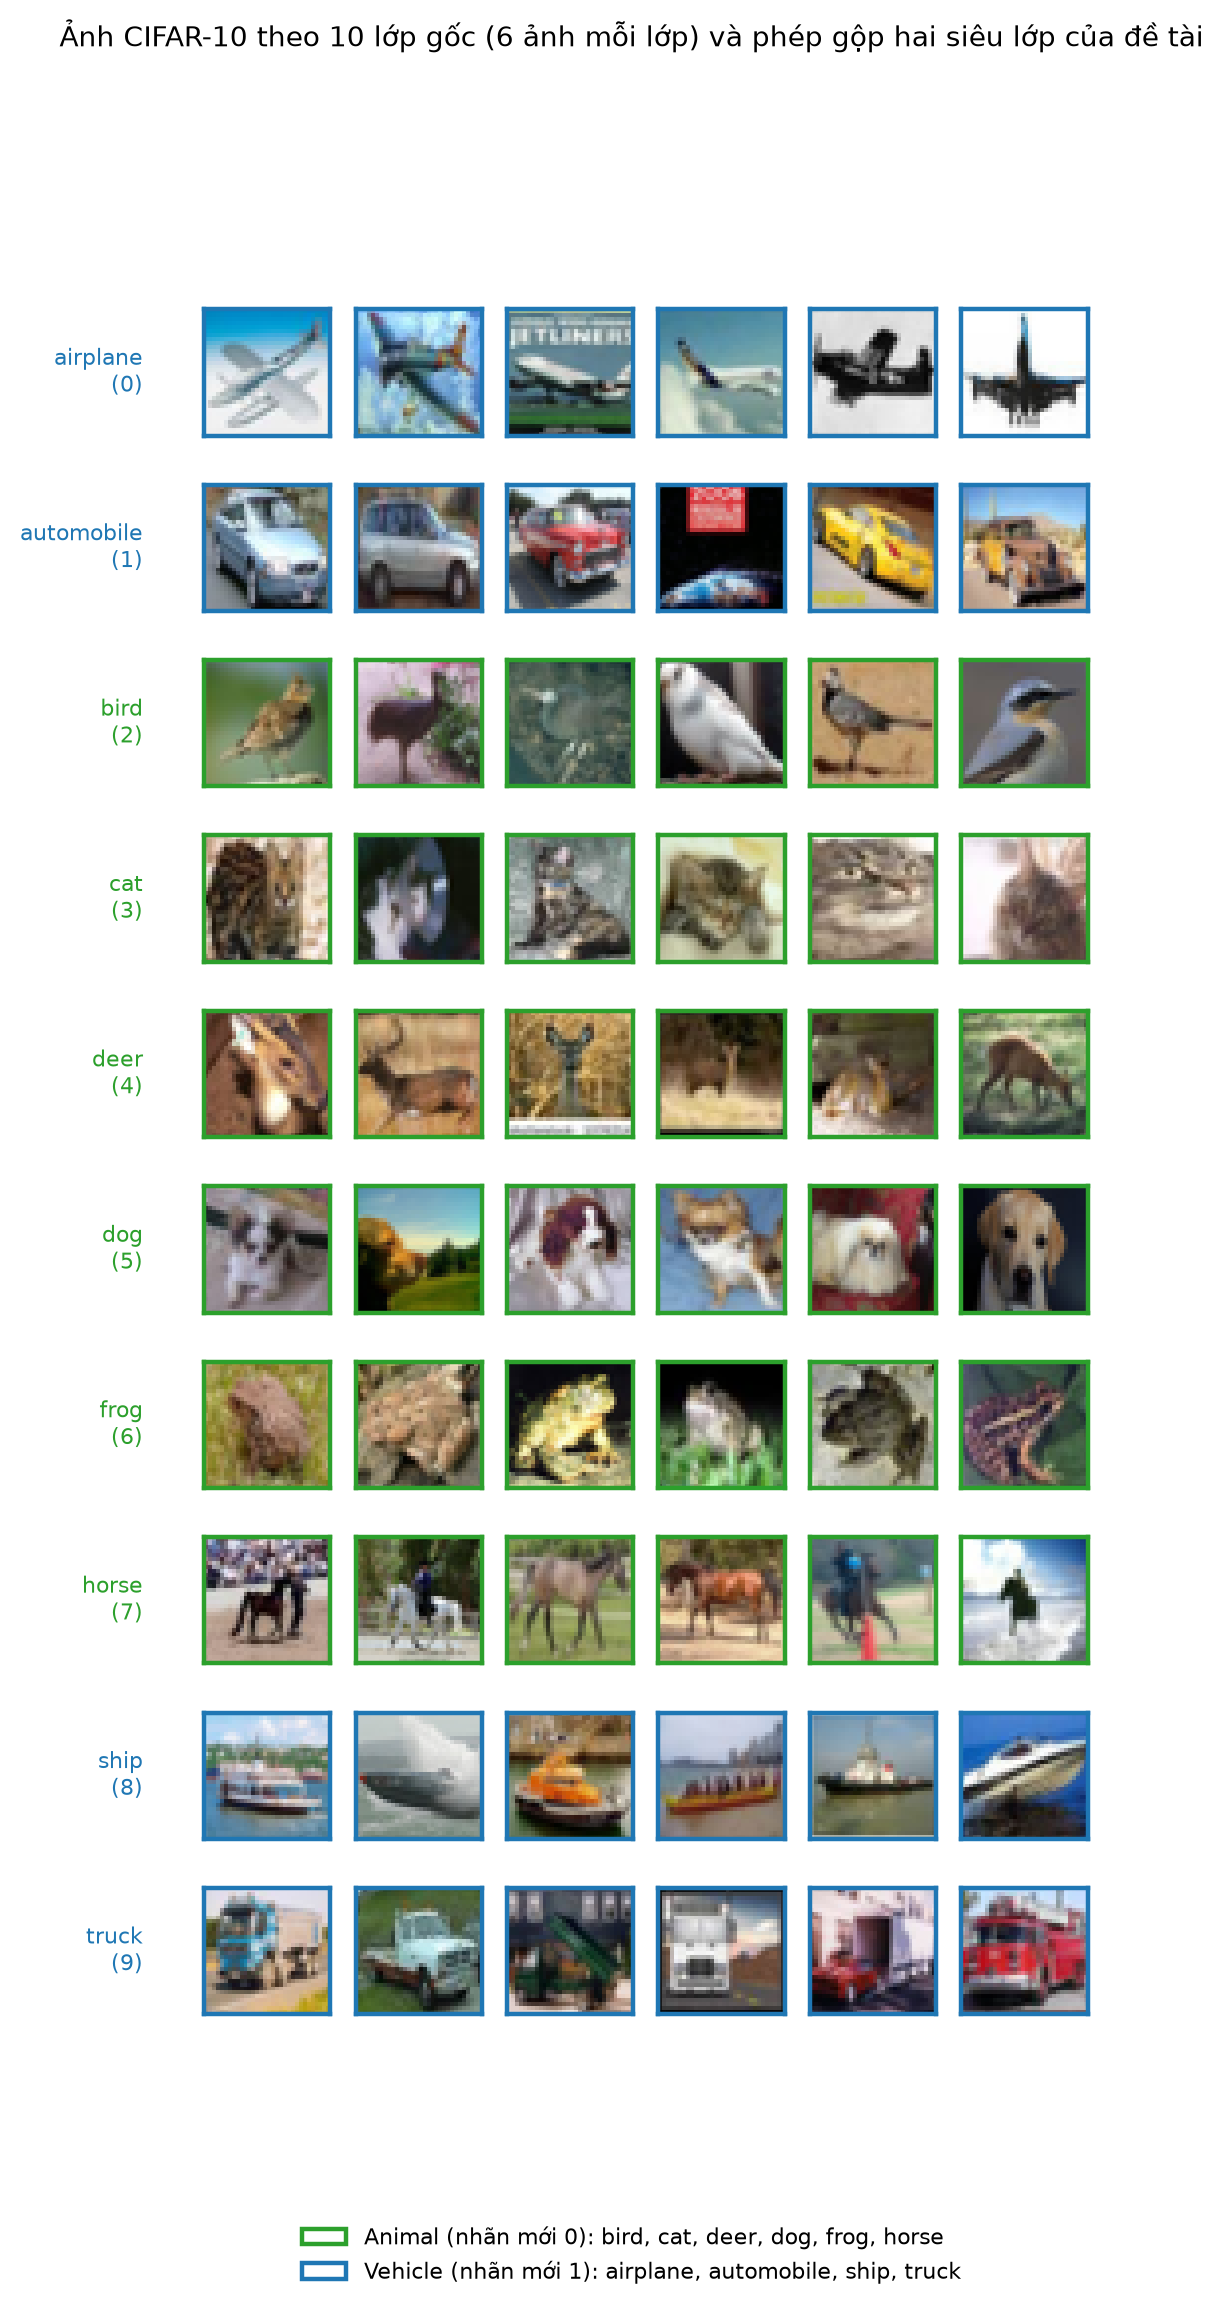
\includegraphics[width=\textwidth]{../results/figures/figA1_dataset_samples.png}
  \caption{Ảnh CIFAR-10 theo 10 lớp gốc (6 ảnh mỗi lớp, lấy ngẫu nhiên với seed 2026) và phép
  gộp hai siêu lớp của đề tài. Khung xanh lá = Animal (nhãn mới 0, gồm 6 lớp gốc);
  khung xanh dương = Vehicle (nhãn mới 1, gồm 4 lớp gốc). Số trong ngoặc là nhãn gốc của
  CIFAR-10.}
  \label{fig:dataset-samples}
\end{figure}

% Sinh tự động — scripts/make_report_data.py
\begin{table}[htbp]
  \centering
  \small
  \begin{tabular}{@{}l r r r r@{}}
    \toprule
    Tập & Tổng số ảnh & Animal & Vehicle & Tỷ lệ Animal \\
    \midrule
    $\Dtrain$ & 45.000 & 27.000 & 18.000 & 60{,}0\,\% \\
    $\Dval$   & 5.000  & 3.000  & 2.000  & 60{,}0\,\% \\
    $\Dtest$  & 10.000 & 6.000  & 4.000  & 60{,}0\,\% \\
    \bottomrule
  \end{tabular}
  \caption{Quy mô và thành phần của ba tập dữ liệu sau phép gộp siêu lớp. Tập test được giữ riêng hoàn toàn và chỉ mở ra ở bước đánh giá cuối cùng.}
  \label{tab:split}
\end{table}

\figref{fig:dataset-distribution} trình bày phân bố lớp trên ba tập. Panel~(a) xác nhận phép chia
phân tầng giữ đúng 5.000 ảnh train và 1.000 ảnh test cho mỗi lớp gốc; panel~(b) cho thấy tỷ lệ
$60/40$ được giữ nguyên trên cả $\Dtrain$, $\Dval$ và $\Dtest$ — điều này là cần thiết để chỉ số
trên validation còn dự báo được cho test; panel~(c) cho thấy ngân sách nhãn thay đổi thế nào
theo ba mức tỷ lệ.

\begin{figure}[htbp]
  \centering
  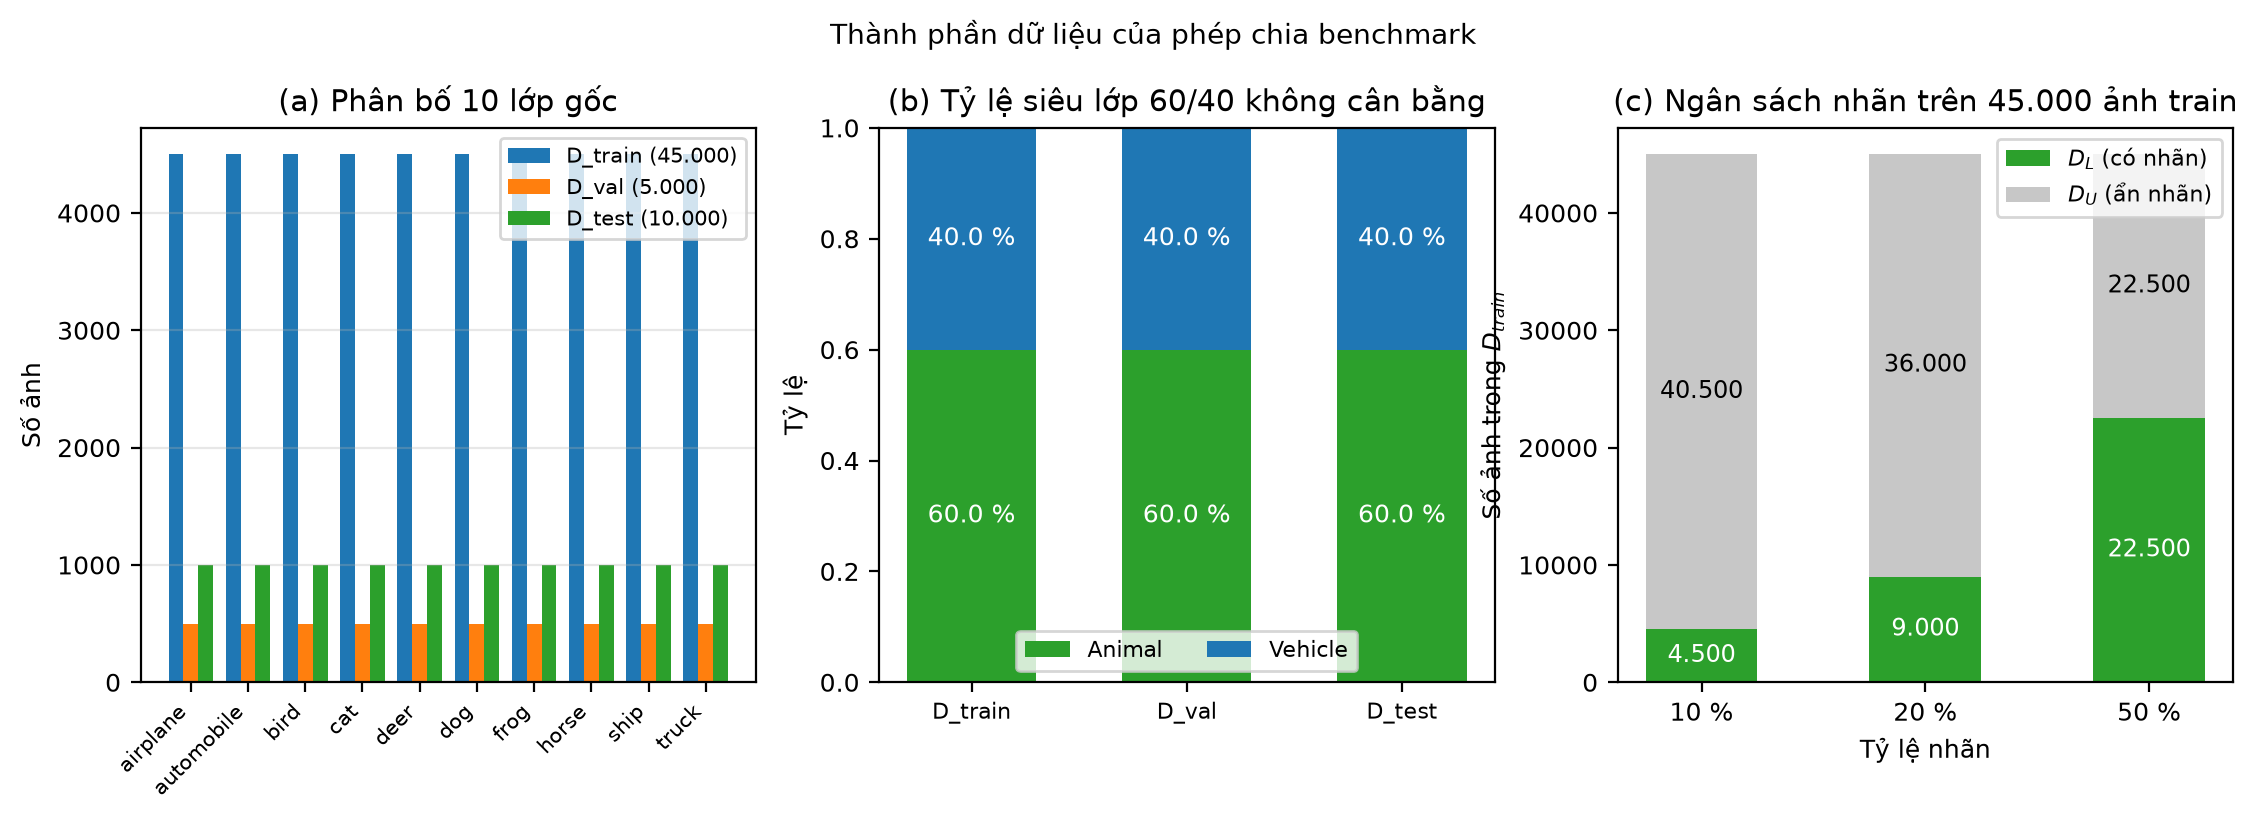
\includegraphics[width=\textwidth]{../results/figures/figA2_class_distribution.png}
  \caption{Thành phần dữ liệu của phép chia benchmark. (a)~Số ảnh mỗi lớp gốc trên ba tập;
  (b)~tỷ lệ hai siêu lớp $60/40$ trên ba tập; (c)~ngân sách nhãn: $\DL$ so với $\DU$ trên
  45.000 ảnh của $\Dtrain$.}
  \label{fig:dataset-distribution}
\end{figure}

\subsection{Chia dữ liệu và ngân sách nhãn}
\label{sec:data-split}

Quy trình chia dữ liệu được đóng băng trước khi huấn luyện và lưu đầy đủ chỉ mục:

\begin{enumerate}[label=\textbf{B\arabic*.},leftmargin=1.4cm,itemsep=3pt]
  \item Dùng seed $2026$ để chia 50.000 ảnh train thành $\Dtrain$ gồm 45.000 ảnh và $\Dval$
        gồm 5.000 ảnh, \emph{phân tầng theo 10 lớp gốc}. Kết quả phân tầng cho
        $\Dval = 3.000$ Animal $+ 2.000$ Vehicle.
  \item Tập test chính thức $\Dtest$ được giữ riêng hoàn toàn, không tham gia bất kỳ bước
        nào của quá trình thiết kế và lựa chọn phương pháp.
  \item Trong mỗi lần lặp $s \in \{42, 43, 44\}$, tạo một thứ tự ngẫu nhiên theo từng lớp gốc
        trên $\Dtrain$, rồi lấy các tập có nhãn \emph{lồng nhau}
        $\DL^{(10\%)} \subset \DL^{(20\%)} \subset \DL^{(50\%)}$.
  \item $\DU = \Dtrain \setminus \DL$ là phần ẩn nhãn; nhãn thật của $\DU$ bị chặn ở mức
        chỉ mục và không bao giờ được đọc trong quá trình huấn luyện.
\end{enumerate}

% Sinh tự động — scripts/make_report_data.py
\begin{table}[htbp]
  \centering
  \small
  \begin{tabular}{@{}l r r r r r@{}}
    \toprule
    Tỷ lệ nhãn & $\DL$ & Animal & Vehicle & $\DU$ & Tổng $\Dtrain$ \\
    \midrule
    10\% & 4.500 & 2.700 & 1.800 & 40.500 & 45.000 \\
    20\% & 9.000 & 5.400 & 3.600 & 36.000 & 45.000 \\
    50\% & 22.500 & 13.500 & 9.000 & 22.500 & 45.000 \\
    \bottomrule
  \end{tabular}
  \caption{Số ảnh huấn luyện theo từng mức tỷ lệ nhãn. $\DL$ là tập có nhãn, $\DU = \Dtrain \setminus \DL$ là phần ẩn nhãn; mọi tỷ lệ được tính trên 45.000 ảnh của $\Dtrain$, không phải trên toàn bộ 60.000 ảnh.}
  \label{tab:label-budget}
\end{table}

Một điểm dễ mắc lỗi cần được nêu rõ: mỗi mức tỷ lệ được tính trên \textbf{45.000 ảnh của
$\Dtrain$}, không phải trên toàn bộ 60.000 ảnh. Ngoài nhãn huấn luyện, 5.000 nhãn validation
được dùng để chọn checkpoint; đây là một khoản chi phí nhãn thật và phải được khai báo riêng
khi thảo luận về mức độ tiết kiệm nhãn. Tổng ngân sách nhãn thực tế của mỗi lượt chạy là
$|\DL| + 5.000$.

\begin{keybox}
\textbf{Quy tắc chống rò rỉ nhãn (được kiểm tra tự động).} Nhãn gốc chỉ phục vụ việc chuẩn bị
phép chia benchmark. Nhãn thật của $\DU$ \emph{không} được đưa vào loss, \emph{không} được
dùng để chọn positive pair, \emph{không} được dùng để huấn luyện bộ phân loại và \emph{không}
được dùng để lựa chọn mô hình. Script \code{scripts/prepare\_data.py} kiểm tra và ghi lại:
không trùng chỉ mục giữa train/validation/test, các tập $\DL$ đúng số lượng của
\tabref{tab:label-budget}, các tập lồng nhau đúng thứ tự, và $\DL \cap \DU = \varnothing$.
Kết quả kiểm tra đầy đủ được lưu trong \code{results/benchmark\_audit.json}.
\end{keybox}

\subsection{Tiền xử lý và sinh nhãn góc xoay}
\label{sec:data-aug}

Hai nhánh sử dụng hai chuỗi biến đổi khác nhau, được mô tả tường minh để tránh hiểu nhầm rằng
cả hai nhánh dùng chung một view.

\paragraph{Nhánh phân loại.}
\code{RandomCrop(32, padding=4)} $\rightarrow$ \code{RandomHorizontalFlip(p=0.5)} $\rightarrow$
chuyển về tensor $[0,1]$ $\rightarrow$ \code{Normalize}. Chuỗi này chỉ áp dụng khi huấn luyện.

\paragraph{Nhánh rotation.}
Dùng ảnh gốc $32 \times 32$ không cắt, chọn $k$ đều trong $\{0,1,2,3\}$, áp dụng
$R_k = $ xoay $90k$ độ ngược chiều kim đồng hồ bằng \code{torch.rot90}, sau đó chuẩn hóa như
trên~\cite{pytorch_rot90}. \textbf{Không} thêm phép xoay hoặc lật nào sau bước gán $k$; nếu
thêm, nhãn $k$ sẽ không còn khớp với biến đổi thực và nhiệm vụ phụ trở nên vô nghĩa.

\paragraph{Validation và test.}
Hai tập này chỉ chuyển tensor và chuẩn hóa, không augmentation ngẫu nhiên.

\figref{fig:views} so sánh trực tiếp ba loại view của \emph{cùng một ảnh}. Sự khác biệt là có
chủ đích: nhánh phân loại cần một view giữ được thông tin ngữ nghĩa (cắt nhẹ, lật ngang), còn
nhánh contrastive cần hai view \enquote{khó} của cùng một ảnh để việc kéo chúng lại gần nhau
thực sự học được bất biến (cắt mạnh, đổi màu mạnh, có thể chuyển xám). Nhánh xoay thì
\textbf{không} được cắt, vì cắt sẽ làm thay đổi góc xoay hiệu dụng và nhãn $k$ không còn khớp
với biến đổi thật.

\begin{figure}[htbp]
  \centering
  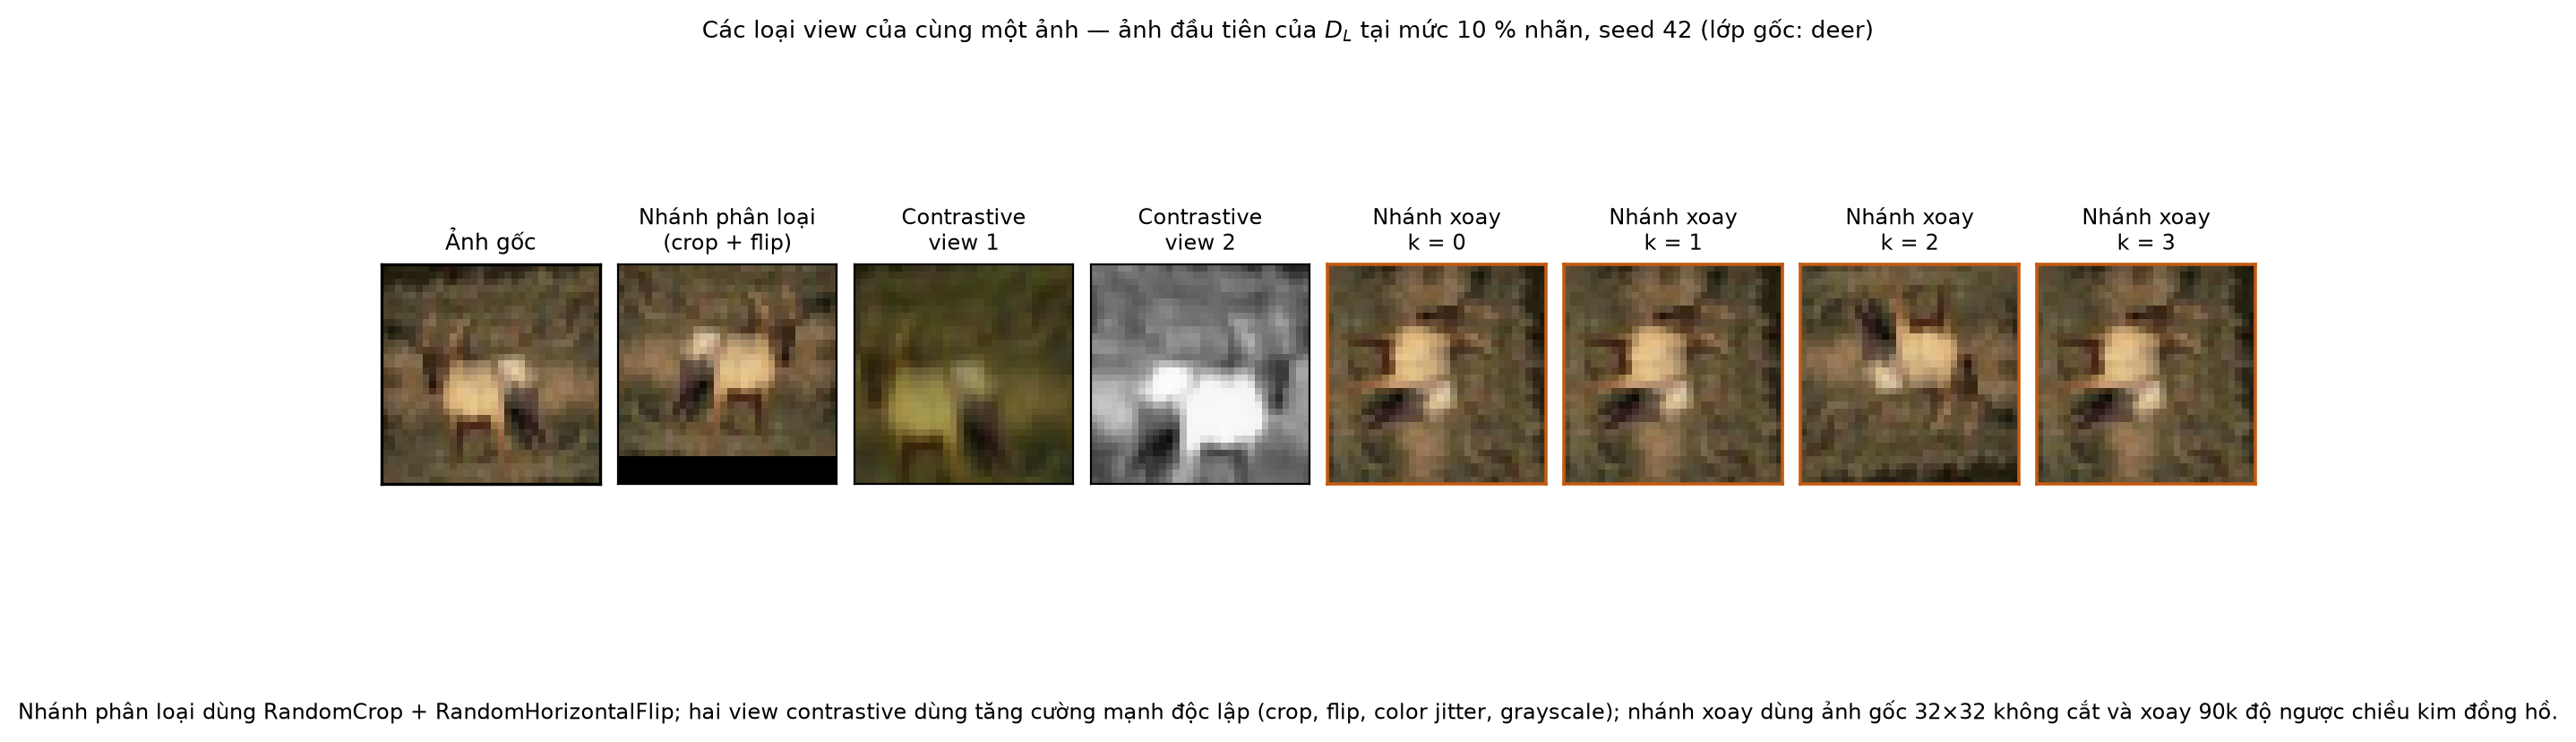
\includegraphics[width=\textwidth]{../results/figures/figA3_views.png}
  \caption{Ba loại view của cùng một ảnh (ảnh đầu tiên của $\DL$ tại mức $10\,\%$ nhãn, seed 42):
  ảnh gốc; view của nhánh phân loại; hai view của nhánh contrastive; và bốn phép xoay $k = 0..3$
  của nhánh phụ. Lưu ý nhánh xoay dùng ảnh \emph{nguyên bản} $32 \times 32$ chứ không dùng ảnh
  đã cắt.}
  \label{fig:views}
\end{figure}

\paragraph{Hằng số chuẩn hóa.}
$\text{mean} = \text{std} = (0{,}5;\ 0{,}5;\ 0{,}5)$. Đây là hằng số được chọn trước, áp dụng
chung cho mọi cấu hình và mọi mức nhãn; giá trị này \emph{không} được ước lượng từ validation
hay test, vì làm như vậy sẽ tạo rò rỉ thông tin giữa các tập.

\begin{figure}[htbp]
  \centering
  \begin{tikzpicture}[
      font=\small,
      box/.style={draw=m8blue,fill=m8light,rounded corners=2pt,minimum height=8mm,
                  minimum width=22mm,align=center,inner sep=3pt},
      sbox/.style={draw=m8teal,fill=green!5,rounded corners=2pt,minimum height=8mm,
                   minimum width=26mm,align=center,inner sep=3pt},
      abox/.style={draw=m8orange,fill=orange!6,rounded corners=2pt,minimum height=8mm,
                   align=center,inner sep=3pt},
      ar/.style={-{Latex[length=2mm]},draw=m8gray,thick},
    ]
    \node[box] (img) {Ảnh gốc\\$3\times32\times32$};

    \node[abox,below left=12mm and 4mm of img] (aug) {RandomCrop\\RandomHorizontalFlip\\Normalize};
    \node[box,below=6mm of aug] (enc1) {Encoder $\enc$};
    \node[sbox,below=6mm of enc1] (sup) {Superclass Head $\gsup$};
    \node[sbox,below=6mm of sup] (out1) {logits $\mathbb{R}^2$};

    \node[abox,below right=12mm and 4mm of img] (rot) {\code{torch.rot90}$(k)$\\$k\sim\mathcal{U}\{0,1,2,3\}$\\Normalize};
    \node[box,below=6mm of rot] (enc2) {Encoder $\enc$};
    \node[sbox,below=6mm of enc2] (head2) {Rotation Head $\grot$};
    \node[sbox,below=6mm of head2] (out2) {logits $\mathbb{R}^4$};

    \draw[ar] (img.south) -- ++(0,-4mm) -| (aug.north);
    \draw[ar] (img.south) -- ++(0,-4mm) -| (rot.north);
    \draw[ar] (aug) -- (enc1);
    \draw[ar] (enc1) -- (sup);
    \draw[ar] (sup) -- (out1);
    \draw[ar] (rot) -- (enc2);
    \draw[ar] (enc2) -- (head2);
    \draw[ar] (head2) -- (out2);

    \begin{scope}[on background layer]
      \node[draw=m8blue,dashed,rounded corners=4pt,fit=(enc1)(enc2),
            inner sep=6pt,label={[m8blue,font=\scriptsize\bfseries]left:{dùng chung}}] {};
    \end{scope}

    \node[abox,right=4mm of out1,minimum width=30mm] (l1) {$\Lsup$ (có nhãn $\DL$)};
    \node[abox,right=4mm of out2,minimum width=30mm] (l2) {$\Lrot$ (không cần nhãn)};
    \draw[ar] (out1) -- (l1);
    \draw[ar] (out2) -- (l2);
  \end{tikzpicture}
  \caption{Luồng huấn luyện hai nhánh của khối chính. Hai nhánh nhận \emph{các view khác nhau}:
  nhánh trên dùng augmentation ngẫu nhiên của ảnh chuẩn, nhánh dưới dùng ảnh đã xoay $90k$ độ.
  Encoder và các lớp BatchNorm được dùng chung, nên thống kê chạy của mạng phụ thuộc vào việc
  có nhánh xoay hay không. Các cấu hình mở rộng \cfg{E3}--\cfg{E6} thêm một nhánh thứ ba đi qua
  cùng encoder rồi qua Projection Head (\secref{sec:contrastive}); ba loại view tương ứng được
  minh họa ở \figref{fig:views}.}
  \label{fig:pipeline}
\end{figure}
